%
% IEEE Transactions on Microwave Theory and Techniques example
% Thibault Reveyrand - http://www.microwave.fr
%
% http://www.microwave.fr/LaTeX.html
% ---------------------------------------



% ================================================
% Please HIGHLIGHT the new inputs such like this :
% Text :
%  \hl{comment}
% Aligned Eq.
% \begin{shaded}
% \end{shaded}
% ================================================



\documentclass[journal]{IEEEtran}

%\usepackage[retainorgcmds]{IEEEtrantools}
%\usepackage{bibentry}
\usepackage{xcolor,soul,framed} %,caption

\colorlet{shadecolor}{yellow}
% \usepackage{color,soul}
\usepackage[pdftex]{graphicx}
\graphicspath{{../pdf/}{../jpeg/}}
\DeclareGraphicsExtensions{.pdf,.jpeg,.png}

\usepackage[cmex10]{amsmath}
%Mathabx do not work on ScribTex => Removed
%\usepackage{mathabx}
\usepackage{array}
\usepackage{mdwmath}
\usepackage{mdwtab}
\usepackage{eqparbox}
\usepackage{url}


% ----------------------------------------------

% Definitions of languages: ------------
\usepackage{listings}
\lstdefinestyle{cStyle}{
  basicstyle=\scriptsize,
  breakatwhitespace=false,
  breaklines=true,
  captionpos=b,
  keepspaces=true,
  numbersep=5pt,
  showspaces=false,
  gobble=4,
  tabsize=4,
  showstringspaces=false,
  showtabs=false,
}
\renewcommand*{\lstlistingname}{Code}

% ----------------------------------------------




\hyphenation{op-tical net-works semi-conduc-tor}

%\bstctlcite{IEEE:BSTcontrol}


%=== TITLE & AUTHORS ====================================================================
\begin{document}
\bstctlcite{IEEEexample:BSTcontrol}
    \title{Otimizations Based on Evolutionary Methods}
  \author{Carlos~Matheus~Barros~da~Silva,~\IEEEmembership{Bachelor Student of ITA}\\Prof. Marcos~Ricardo~Omena~de~Albuquerque~Máximo}


% The paper headers
\markboth{INSTITUTO TECNOLÓGICO DE AERONÁUTICA, APRIL~2019
}{Otimizations Based on Evolutionary Methods}


% ====================================================================
\maketitle



% === ABSTRACT ==============================================================
% ============================================================================
\begin{abstract}
%\boldmath
In this paper is the evaluation of an Evolutionary Optimization Method denominated Simple Evolution Strategy (SES) and its performance is compared with the Covariance Matrix Adaptation Evolution Strategy (CMA-ES).

The results shows that since the SES approach not so sofisticated it needs a larger population in order to achieve as good resuls as CMA-ES gets with a smaller population.

Although in some cases they performed similary, and with a small increase in population in SES makes it perform as good as CMA-ES, and in some cases SES with a larger population performed better then CMA-ES. With this, therefore, SES is a simple and effective optimization method.

% === KEYWORDS ===============================================================
% ============================================================================
\begin{IEEEkeywords}
    Simple Evolution Strategy, SES, Covariance Matrix Adaptation Evolution Strategy, CMA-ES, optimization
\end{IEEEkeywords}
\end{abstract}

\IEEEpeerreviewmaketitle

% ====================================================================
% ====================================================================
% ====================================================================


% === I. INTRODUCTION ========================================================
% =============================================================================
\section{Introduction}

\IEEEPARstart{I}{n} computer science, an evolution strategy (ES) is an optimization technique based on ideas of evolution. It belongs to the general class of evolutionary computation or artificial evolution methodologies.

Usualy Evolution strategies use natural problem-dependent representations, and primarily mutation and selection, as search operators. In common with evolutionary algorithms, the operators are applied in a loop. An iteration of the loop is called a generation. The sequence of generations is continued until a termination criterion is met.

\subsection{Simple Evolution Strategy}

In this paper the Simple Evolution Strategy (SES) approach relies on a covariance matrix and a mean. For each itetation the algorithm makes a uniform sampling with the mean and covariance matrix and then gets the $\mu$ best positions and makes the mean of its position be the next mean and uptate the covariance matrix. This SES behavior can be described with the Equation \ref{equation:esemean} and Equation \ref{equation:eseconvariancematrix}.

\begin{equation}
    \label{equation:esemean}
    m^{g+1} = \frac{1}{\mu} \sum_{i=1}^{\mu} S_{i:\lambda}^{g+1}
\end{equation}

\begin{equation}
    \label{equation:eseconvariancematrix}
    C^{g+1} = \frac{1}{\mu} \sum_{i=1}^{\mu} (S_{i:\lambda}^{g+1} - m^g) (S_{i:\lambda}^{g+1} - m^g)^T
\end{equation}

\subsection{Covariance Matrix Adaptation Evolution Strategy}

CMA-ES stands for covariance matrix adaptation evolution strategy. Evolution strategies (ES) are stochastic, derivative-free methods for numerical optimization of non-linear or non-convex continuous optimization problems. They belong to the class of evolutionary algorithms and evolutionary computation. An evolutionary algorithm is broadly based on the principle of biological evolution, namely the repeated interplay of variation (via recombination and mutation) and selection: in each generation (iteration) new individuals (candidate solutions, denoted as $x$) are generated by variation, usually in a stochastic way, of the current parental individuals. Then, some individuals are selected to become the parents in the next generation based on their fitness or objective function value $f(x)$. Like this, over the generation sequence, individuals with better and better $f$-values are generated.

In an evolution strategy, new candidate solutions are sampled according to a multivariate normal distribution in ${R}^{n}$. Recombination amounts to selecting a new mean value for the distribution. Mutation amounts to adding a random vector, a perturbation with zero mean. Pairwise dependencies between the variables in the distribution are represented by a covariance matrix. The covariance matrix adaptation (CMA) is a method to update the covariance matrix of this distribution. This is particularly useful if the function $f$ is ill-conditioned.

Adaptation of the covariance matrix amounts to learning a second order model of the underlying objective function similar to the approximation of the inverse Hessian matrix in the Quasi-Newton method in classical optimization. In contrast to most classical methods, fewer assumptions on the nature of the underlying objective function are made. Only the ranking between candidate solutions is exploited for learning the sample distribution and neither derivatives nor even the function values themselves are required by the method.

Two main principles for the adaptation of parameters of the search distribution are exploited in the CMA-ES algorithm.

First, a maximum-likelihood principle, based on the idea to increase the probability of successful candidate solutions and search steps. The mean of the distribution is updated such that the likelihood of previously successful candidate solutions is maximized. The covariance matrix of the distribution is updated (incrementally) such that the likelihood of previously successful search steps is increased. Both updates can be interpreted as a natural gradient descent. Also, in consequence, the CMA conducts an iterated principal components analysis of successful search steps while retaining all principal axes. Estimation of distribution algorithms and the Cross-Entropy Method are based on very similar ideas, but estimate (non-incrementally) the covariance matrix by maximizing the likelihood of successful solution points instead of successful search steps.

Second, two paths of the time evolution of the distribution mean of the strategy are recorded, called search or evolution paths. These paths contain significant information about the correlation between consecutive steps. Specifically, if consecutive steps are taken in a similar direction, the evolution paths become long. The evolution paths are exploited in two ways. One path is used for the covariance matrix adaptation procedure in place of single successful search steps and facilitates a possibly much faster variance increase of favorable directions. The other path is used to conduct an additional step-size control. This step-size control aims to make consecutive movements of the distribution mean orthogonal in expectation. The step-size control effectively prevents premature convergence yet allowing fast convergence to an optimum.

% ==========================================================================
\section{Simple Evolution Strategy (SES) Implementation}

The implementation was based on the file \textit{simple evolution strategy}. The essence of the implementation is on \textit{SimpleEvolutionStrategy} Class and on \textit{tell} method.

The \textit{tell} method updates the mean and the coraviance matrix of SES and its implementation can be seen on Code \ref{code:tell}.

\lstinputlisting[
    language=python,
    caption={Code of \textit{tell} method},
    label={code:tell},
    style=cStyle,
    firstline=39,
    lastline=58
]{./../code/simple_evolution_strategy.py}

\section{SES performance analysis}

In this analysis was used four functions: Translated Sphere, Ackley, Schaffer function, Rastrigin (2D).

SES performed very well in most case finding the minimum global. In Translated Sphere and Ackley using the parameters defined on the file test evolution strategy the result of SES for these two test functions was similar to the result of CMA-ES.

On the images Image \ref{img:test_evolution_strategy-translated_sphere-SES} and Image \ref{img:test_evolution_strategy-ackley-SES} is shown the convergence of SES on these two test functions. And for these two tests the codes from Code \ref{code:translated_sphere_fitness} to Code \ref{code:ackley_samples} shown its fitness and sample progresses.

\begin{figure}
  \begin{center}
  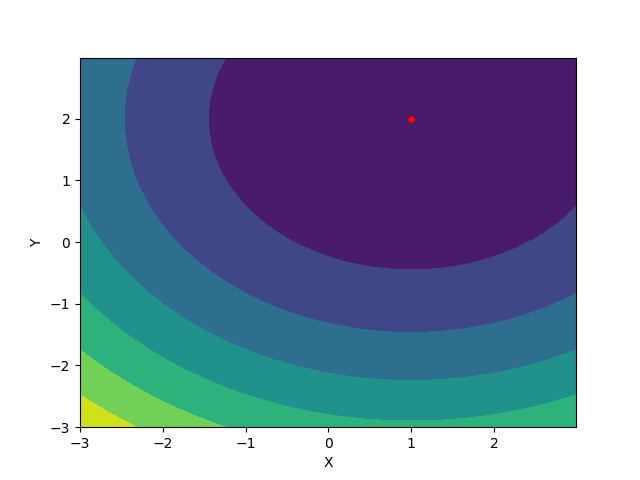
\includegraphics[width=2.8in]{./../code/test_evolution_strategy_results/test_evolution_strategy-translated_sphere-SES.png}
  \caption{Convergence of SES on Translated Sphere function}
  \label{img:test_evolution_strategy-translated_sphere-SES}
  \end{center}
\end{figure}

\lstinputlisting[
    language=python,
    caption={First 10 and last 10 fitness results of SES on Translated Sphere function},
    label={code:translated_sphere_fitness},
    style=cStyle,
]{./../code/test_evolution_strategy_results/test_evolution_strategy-translated_sphere-SES_fitness_short.txt}

\lstinputlisting[
    language=python,
    caption={First 10 and last 10 samples of SES on Translated Sphere function},
    label={code:translated_sphere_samples},
    style=cStyle,
]{./../code/test_evolution_strategy_results/test_evolution_strategy-translated_sphere-SES_history_sample_short.txt}

\begin{figure}
  \begin{center}
  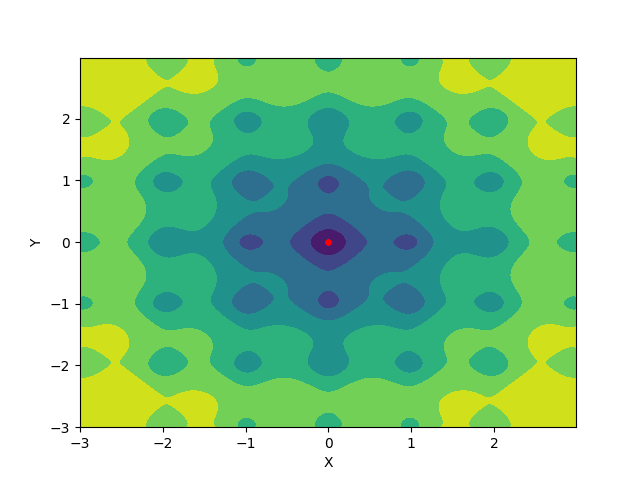
\includegraphics[width=2.8in]{./../code/test_evolution_strategy_results/test_evolution_strategy-ackley-SES.png}
  \caption{Convergence of SES on Translated Sphere function}
  \label{img:test_evolution_strategy-ackley-SES}
  \end{center}
\end{figure}

\lstinputlisting[
    language=python,
    caption={First 10 and last 10 fitness results of SES on Ackley function},
    label={code:ackley_fitness},
    style=cStyle,
]{./../code/test_evolution_strategy_results/test_evolution_strategy-ackley-CMAES_fitness_short.txt}

\lstinputlisting[
    language=python,
    caption={First 10 and last 10 samples of SES on Ackley function},
    label={code:ackley_samples},
    style=cStyle,
]{./../code/test_evolution_strategy_results/test_evolution_strategy-ackley-CMAES_history_sample_short.txt}

But it was verified as well that for more dificult functions like Schaffer function and Rastrigin (2D) the SES can easily be stocked on a local minimum. The images

\begin{figure}
  \begin{center}
  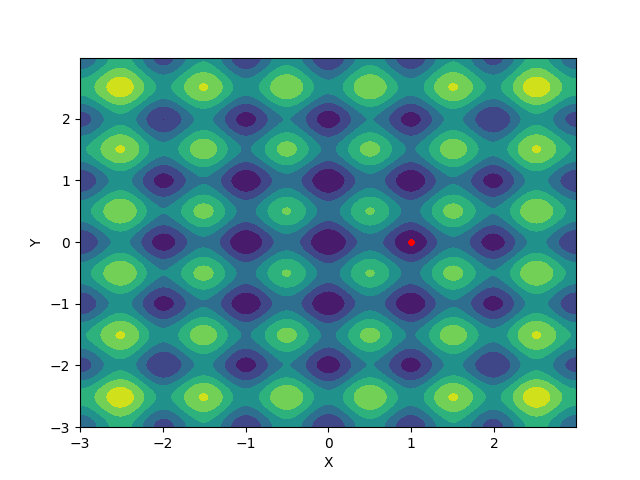
\includegraphics[width=2.8in]{./../code/test_evolution_strategy_results/test_evolution_strategy-rastrigin-SES.png}
  \caption{Convergence of SES on Rastrigin (2D) function}
  \label{img:test_evolution_strategy-rastrigin-SES}
  \end{center}
\end{figure}

\lstinputlisting[
    language=python,
    caption={First 10 and last 10 fitness results of SES on Rastrigin (2D) function},
    label={code:translated_sphere_fitness},
    style=cStyle,
]{./../code/test_evolution_strategy_results/test_evolution_strategy-translated_sphere-SES_fitness_short.txt}

\lstinputlisting[
    language=python,
    caption={First 10 and last 10 samples of SES on Rastrigin (2D) function},
    label={code:translated_sphere_samples},
    style=cStyle,
]{./../code/test_evolution_strategy_results/test_evolution_strategy-rastrigin-SES_history_sample_short.txt}

\begin{figure}
  \begin{center}
  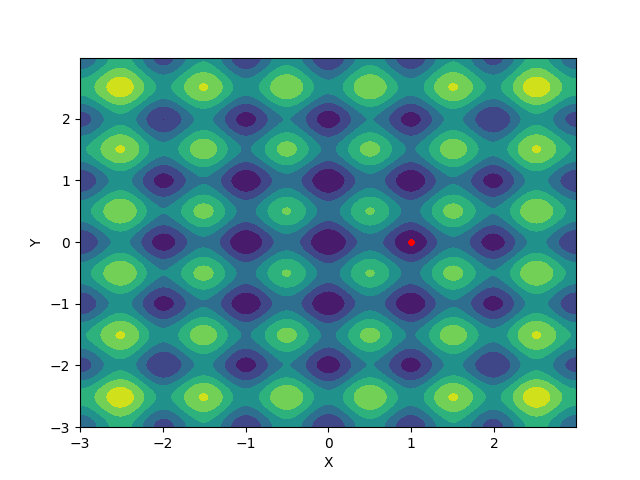
\includegraphics[width=2.8in]{./../code/test_evolution_strategy_results/test_evolution_strategy-rastrigin-SES.png}
  \caption{Convergence of SES on Rastrigin (2D) function}
  \label{img:test_evolution_strategy-rastrigin-SES}
  \end{center}
\end{figure}

\lstinputlisting[
    language=python,
    caption={First 10 and last 10 fitness results of SES on Rastrigin (2D) function},
    label={code:rastrigin_fitness},
    style=cStyle,
]{./../code/test_evolution_strategy_results/test_evolution_strategy-rastrigin-CMAES_fitness_short.txt}

\lstinputlisting[
    language=python,
    caption={First 10 and last 10 samples of SES on Rastrigin (2D) function},
    label={code:rastrigin_samples},
    style=cStyle,
]{./../code/test_evolution_strategy_results/test_evolution_strategy-rastrigin-CMAES_history_sample_short.txt}

\section {Conclusion}

It was clear, therefore, that \textit{PSO} method was implemented successfully. And by analyzing its results, it can be seen that \textit{PSO} has a fast conversion, but it does not converge to something necessarily great.

In fact, it finds local maximums and can easily be stocked on it. But for many cases, it is good enough. In the case test, the solution found was able to complete the entire track in about 11 seconds, that is, it was really fast and precise at the same time.

As it is possible to see on the on Figure \ref{img:initial_line_follower_solution} and Figure \ref{img:initial_line_follower_solution} that at initials iterations the parameters are really bad, and with the time after many iterations it has a convergence to something good.

\vfill
\end{document}
